\section{Security Analysis}
\label{sec:securityAnalysis}

In this section, we will informally analyze the security of \name. We divide the security analysis into two parts based on two security properties: interity and confidentiality.

\subsection{Integrity}
\label{sec:securityAnalysis:integrity}

First we look into the integrity property.

\myparagraph{Modifying IO operations} As only the \device can interact with the overlaid UI, the attacker can not manipulate the IO operations with the overlaid UI. Moreover, the attacker cannot submit arbitrary data to the remote server because the latter accepts only inputs signed by the \device.


\myparagraph{Early form submission} This attack is not possible as the input devices (both mouse and keyboard) are connected to the \device, and only the \device can interact with the overlaid UI. This makes it impossible for the attacker to emulate a click on the overlaid part of the screen.  


\myparagraph{Attack on the mouse pointer tracking and overlay} 
The attacker may try to defeat the \name pointer tracking and overlay mechanism described in Section~\ref{sec:systemDesign:analysis} by introducing a malicious pointer that is visually more appealing to the user. Note that the \device overlaid mouse pointer is prominent and hard to miss. One can visualize it as an arms race between the attacker and the \device to grab the user's attention. We argue that this is a suboptimal strategy for the attacker as both of the pointers will be visible on the screen that causes suspicion to the user. Also, when the real mouse pointer enters the overlaid area, the untrusted part, including the malicious mouse pointer, will be hidden by the focusing mechanism. Hence, we can conclude that executing clickjacking-like attacks is not possible in \name.


\myparagraph{Replay attack} The remote server adds a random identifier (\texttt{id}) in the form specification alongside the signature. With this identifier, the server keeps track of the user input. When the server receives a form submission data, it first checks if the user submitted with the same identifier sent by the server. Otherwise, the server rejects the data. 


\myparagraph{Not rendering QR code} The host may deny sending the QR code over the HDMI channel. We consider this to be a denial of service and does not compromise the integrity of the IO data. 


\myparagraph{Redirection} The attacker could redirect the user to a phishing website that renders visually identical UI to that of the legitimate website. A redirection attack cannot break the integrity of the input because a legitimate remote server always requires the signed input from the user. Without a valid signed specification, the \device never renders an overlay or sign any input. 

\myparagraph{Malicious instruction on the screen} The attacker may put a malicious instruction/label on the untrusted part of the screen to influence user inputs. However, when the user starts interacting with the overlaid UI, the default focusing mechanism (Lightbox) highlights only the secure UI and hides the rest of the screen. 
%The user attention focusing mechanisms enable the user to distinguish the trusted part of the screen from the untrusted part.


\myparagraph{Replication of Lightbox} The attacker can replicate the lightbox on any part of the screen. However, this does not compromise the integrity of the input as the legitimate remote server only accepts signed input from the \device. 


\myparagraph{Multiple HIDs} The attacker can emulate multiple HIDs to avoid the tracking of the mouse pointer. However, this attack is ineffective as the \device only tracks the mouse pointer that is connected to it (over USB interface). 


\myparagraph{BadUSB} BadUSB~\cite{badUSB} is out-of-scope of this paper as in the attacker model (Section~\ref{sec:approach:systemAttackerModel}), we assume that all the IO devices that are connected to the \device are trusted.

\myparagraph{Mouse acceleration/updates} The attacker can change the mouse acceleration or provide erratic mouse updates on the screen. Such manipulations only cause the \device to lose track of the mouse pointer and stop relaying the mouse signal to the host altogether. The \device uses the acceleration parameters from the default \texttt{libUSB} driver to cope with the mouse acceleration. Hence, such manipulation does not affect security.

\myparagraph{Malicious QR codes} The attacker may put fake QR codes on the webpage. Note that the \device verifies the signature from the HTML forms to check the integrity using the pre-configured or white-listed server certificate. This way, the \device does not render any overlays from malicious QR codes.


\subsection{Confidentiality}
\label{sec:securityAnalysis:confidentiality}

\myparagraph{Redirection} The attacker could redirect the user to a phishing website that renders visually identical UI to that of the legitimate website. Redirection compromises the confidentiality of user inputs only when the user does not trigger the SAS mechanism. The \device is only activated when it detects specifications signed from the whitelisted (maintained in the memory) servers.
%Note that the \device contains a whitelist of the remote server addresses and their corresponding certificates. The \device is only activated when it detects specifications signed from the whitelisted servers.
%as the confidentiality of inputs requires the user to manually trigger the SAS to detect any sensitive UI elements that are overlaid by the \device.


\myparagraph{Fake SAS instructions} The attacker may put fake instructions on the screen that attempt to trick the user into typing a false SAS sequence and then revealing her sensitive information to the attacker. This attack is not possible as long as the user follows the instructions it received from the issuer of the \device and only types in secrets after using the correct SAS value (such as \texttt{Ctr+Alt+Del}). Recall from Section~\ref{sec:confidentiality:SAS} that the SAS value is defined by the issuer of the \device and that the SAS keystrokes are always first intercepted by the \device. (The user is expected to trigger the SAS only when there exists a QR code on the screen that is correctly signed by the remote server. In case there is no QR code or a malformed QR code on the screen, the \device warns the user.)


\myparagraph{Side-channel leakages} Even though, the \device ensures that no mouse or keyboard event arrives at the untrusted host when the user executes some operation over the overlaid UI, one can not rule out all side-channel leakages. Depending on the application, the amount of time that the user spends or the entry/exit position of the mouse pointer may reveal some information to the attacker. 
\device could allow the remote server to specify additional policies in the specification to prevent such side-channel attacks, e.g., a minimum amount of time that the device should not forward any event to the host after the user enters the overlay. We leave as future work defining such policies and integrating them on \name.
%However, for fixed-length inputs such as the pin codes or credit card details, do not leak any information about the input.


\myparagraph{Mode Switching} The host could remove the QR code when the user is typing confidential data in the sensitive form. The absence of the QR code makes the \device to assume that the secure session has ended, and the \device forwards the plaintext keystrokes and mouse movement to the host. To prevent the leakage of the input data, the \device continues to overlay and operate on the overlay until the user clicks submit or cancel (or any UI element that has a \texttt{trigger}  capability). This way, the \device locks the UI from the attacker until the user finishes her session.

\subsection{Attacks toward \device} 
\label{sec:securityAnalysis:device}

In \name trust model, we assume that the \device is trusted. However, in the real-world, embedded systems are often vulnerable to attacks as the attacker can use the connection interfaces to reprogram the \device. It is also possible to develop the \device using formally verified languages such as embedded Rust. However, we consider making a security-hardened \device is engineering intensive and out-of-scope of this paper. 


\myparagraph{Downgrade attack} The host can block the initial QR code from the server to the \device. By doing so, the host forces the server to downgrade the security of the webpage, i.e., not serving the \name JS. For integrity, this is not a security threat as the server does not accept any input from the host that is not signed by the \device. Hence, the downgrade attack works as a denial of service, which is out-of-scope of this paper.
%The fallback mechanism, i.e., the case where the user does not have the \device, is outside the scope of this work because it is specific to the policy of service providers. E.g., a bank could issue a new \device for the user, while an online shopping site could allow the user to enroll a new \device or allow access only to nonsensitive functionalities. 


\subsection{Proof for IO Integrity}
\label{sec:securityAnalysis:proof}

In this section, we provide a formal proof of the following property: \emph{without protecting both input and output integrity, none of them can be achieved}. 


%\subsection{Interaction Protocol} 
%\label{appendix:security:protocol}

\myparagraph{Interaction protocol}

To simplify the proof, we model the interaction between the user, the host, and the remote server as a finite state automaton (FSA).
The interactions between the server (\server), the user (\user) and host (\host) are depicted in the FSA in Figure~\ref{fig:fsm}.

\begin{figure}[h!]
\begin{center}
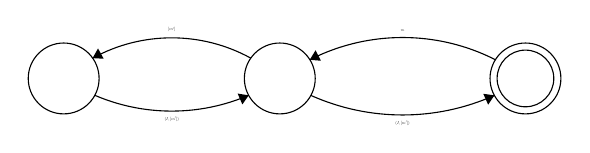
\begin{tikzpicture}[scale=0.15]
\tikzstyle{every node}+=[inner sep=0pt]
\draw [black] (66,-23.1) circle (3);
\draw (66,-23.1) node {\server};
\draw [black] (66,-23.1) circle (2.4);
\draw [black] (45.2,-23.1) circle (3);
\draw (45.2,-23.1) node {\host};
\draw [black] (26.9,-23.1) circle (3);
\draw (26.9,-23.1) node {\user};
\draw [black] (47.743,-21.516) arc (116.95563:63.04437:17.332);
\fill [black] (47.74,-21.52) -- (48.68,-21.6) -- (48.23,-20.71);
\draw (55.6,-19.13) node [above] {$m$};
\draw [black] (29.352,-21.382) arc (118.8302:61.1698:13.89);
\fill [black] (29.35,-21.38) -- (30.29,-21.43) -- (29.81,-20.56);
\draw (36.05,-19.16) node [above] {$[m']$};
\draw [black] (42.565,-24.526) arc (-66.78269:-113.21731:16.527);
\fill [black] (42.57,-24.53) -- (41.63,-24.38) -- (42.03,-25.3);
\draw (36.05,-26.36) node [below] {$(I,[m'])$};
\draw [black] (63.369,-24.535) arc (-65.91058:-114.08942:19.034);
\fill [black] (63.37,-24.53) -- (62.43,-24.4) -- (62.84,-25.32);
\draw (55.6,-26.69) node [below] {$(I,[m'])$};
\end{tikzpicture}
\end{center}
\caption[\name protocol FSM]{Finite state machine that depicts the interaction between the user (\user), host (\host) and the server (\server).}
\label{fig:fsm}
\end{figure}

The server \server sends a message $m$ to the host \host. As we consider a setting where the user \user interacts with \server over browser through web UI. Hence we assume $m$ to be the HTML, JavaScript, and other data send from \server as HTTP payloads. We denote $[m]$ to be the render of $m$ by the \host. As \host is malicious, it can transform $m$ to $m'$. Note that this transformation from the message to render to the user's display is a public knowledge and is deterministic. Hence, for a message $m'$, where $m\neq m'$, then given the corresponding renders $[m']$ and $[m]$, \server can determine that $[m]\neq [m']$. We denote the user input to be $I$, which corresponds to a specific $[m]$. 
%Note that the communication channel between \server to \user is neither authenticated, neither confidential. But the communication channel from \user and \server is authenticated. 
In this model, we simplify the user input by assuming that the \user only provides an input $I$ only after observing a message transformation $[m]$. The user provides both her input $I$ and transformation $[m']$ observed by her to \host. The interaction loop between \host and \user can continue until \user finishes her input. After every input \host hands over new message transformation to \user (either result of the input or new message from \server or both). This simulates the changes in the web UI when the user starts interact with it e.g., input feedback. Once the user provides all her inputs, \host send the sequence of pairs $(I, [m'])$ to \server.

To smmarize the interaction protocol above, we define these two mappings as the following:

\begin{align*}
\texttt{Input()}&:[m]\rightarrow I \\
\texttt{Transform()}&:m,I\rightarrow [m'],\ \exists i\in I:i=\phi
\end{align*}
Both of them are \emph{bijective}.

One trace of the protocol transcript mentioned above is depicted in Figure~\ref{fig:protocol}. As described in the FSM (refer to Figure~\ref{fig:fsm}), \server receives a trace of message transformations $([m']_1,[m']_2,\ldots,[m']_n)$ and corresponding inputs ($I_1,I_2,\ldots,I_n$). From these traces \server could determine of all the $[m']_i$ are in proper form by verifying if $[m]_i=[m']_i$.

Given the interaction protocol, we can now formally define the definitions in this chapters such as the input intergity and output intergerity as the following:

\begin{figure}[t]
\begin{center}
\tikzset{
  every picture/.append style={
    transform shape,
    scale=1
  }
 }
\begin{sequencediagram}
\newinst{u}{\user}
\newinst[3]{h}{\host}
\newinst[3]{s}{\server}
\mess{s}{$m$}{h}
\mess{h}{$[m']_1$}{u}
\mess{u}{$I_1,[m']_1$}{h}
%\mess{h}{$[m']_2$}{u}
%\mess{u}{$I_2,[m']_2$}{h}
\mess{h}{...}{u}
\mess{u}{...}{h}
\mess{h}{$[m']_n$}{u}
\mess{u}{$I_n,[m']_n$}{h}
\mess{h}{$I_1,I_2,...,I_n$}{s}
\mess{h}{$[m']_1,[m']_2,...,[m']_n$}{s}
\end{sequencediagram}
\end{center}
\caption[\name protocol transcript]{Protocol transcript between the \server, \user and \host that shows one trace from the FSM depicted in Figure~\ref{fig:fsm}.}
\label{fig:protocol}
\end{figure}


\begin{definition}{\textbf{Input integrity}}
\label{def:inputIntegrity}

Assume that \server handed a message $m$ to \host where the proper message transformation is $[m]$. The host changes the message transformation to $[m']$ where $[m']\neq [m]$. We also define correct \user input to be $I$ when \host sends a correct message transformation $[m]$ to \user. We define input integrity as the property where the \server does not accept input $I'$ where $I'\neq I$from \user if the \host changes the message transformation.
\end{definition}

\begin{definition}{\textbf{Output integrity}}
\label{def:outputIntegrity}
Assume that \server handed a message $m$ to \host where the proper message transformation is $[m]$. Output integrity defines that in all circumstances, \user receives the correct message transformation $[m]$ from \host.
\end{definition}

\myparagraph{Verification process} After receiving all the traces, \server checks $\forall i=1\ldots n$ $$[m']_i =^? \texttt{Transform}(m_{i-1}, I_{i-1})$$ where $I_0=\phi$.

\begin{lemma}
\label{theorem:th1}
If \user does not send all the transformations till $[m']_i$ corresponding to the input $I_i$, input integrity can not be achieved. 
\end{lemma}

\begin{proof}
If \user does not attach all the transformation till $[m']_i$, i.e., $$[m']_1, [m']_2, \ldots, [m']_{x+1}, [m']_x, [m']_{x-1}, \ldots, [m']_{i-1}, [m']_i$$  corresponding to inputs $I_1, I_2,\ldots, I_{x-1}, I_x, I_{x-1}, \ldots, I_{i-1}, I_i$, then the server can not verify all the transformations corresponding to the input. \host could modify a specific $[m]_x$ to influence \user input. Hence, the following verification will be missing:
$$[m']_x=^?\texttt{Transform}({m'}_{x-1}, I'_{x-1})$$
Where the \host changes message $m$ to $m'$ influence the the user to change her input from $I_{x-1}$ to $I_{x-1}$. Hence input integrity can not be achieved.
\end{proof}

\begin{lemma}
\label{theorem:th2}
If the channel from \user and \server is not authenticated, input integrity is not achievable. But the channel from \server to \user does not require to be secure as long a \user provides the message transformation $[m']_i$ corresponding to every input $I_i$.
\end{lemma}

\begin{proof}
The proof is trivial. If the channel from \user to \server is not authenticated, any input provided by \user can be manipulated by \host without a trace. Hence input integrity is not achievable. As long as \user sends message transformation along with the input, a manipulated message transformation bt \host would be detectable by \server (see Lemma~\ref{theorem:th1}).
\end{proof}

\begin{lemma}
\label{theorem:th3}
Ensuring output integrity also ensures input integrity provided there is an authenticated channel from \user to \server.
\end{lemma}

\begin{proof}
This proof is also trivial. As we describe in the Definition~\ref{def:inputIntegrity} and~\ref{def:outputIntegrity}, if all the message transform from \host $[m']=[m]$, and \host always executes \texttt{Transform()} properly, the input integrity is preserved. As \name ensures output integrity and all the input from the user is signed by the \device, \name preserves input integrity. 
\end{proof}


